\begin{quote}\small\textbf{观课提示}\quad 对比确定来源与公平二元来源，区分理想平均长度和单符号整数码长。

\href{https://www.youtube.com/watch?v=l6DKRf-fAAM}{原课程视频}\quad\href{https://vitael04213.github.io/3blue1brown-notes/lessons/entropy.html}{本节网页与媒体}\quad\href{https://vitael04213.github.io/3blue1brown-notes/lab.html\#entropy}{参数实验}
\end{quote}
\begin{figure}[htbp]\centering
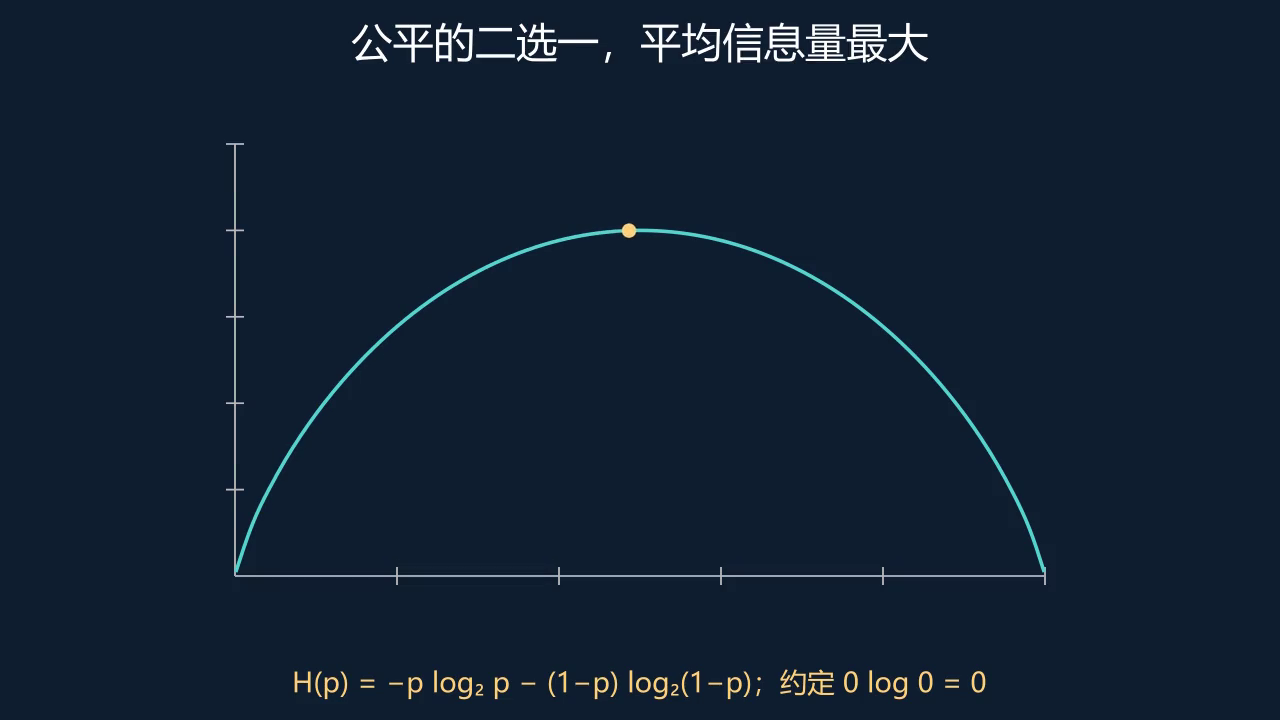
\includegraphics[width=0.98\linewidth]{figures/Entropy.png}
\caption{二元熵在公平概率处达到一位；接近确定事件时下降。本项目原创 Manim 动画关键帧；完整动画与操作入口见本节网页。}
\end{figure}
